\chapter{統計を用いた画像再構成手法の改善}
\newpage
\section{概要}
本章では, 骨のような下肢組織の断層画像取得の際の精度の向上のための統計的処理の検討を述べる.
\section{下肢組織の構造}
下肢組織は, 大きく分けて上腿と下腿の2つに分けられる(\figref{kashisoshiki}). 上腿には大腿骨が, 下腿には脛骨および腓骨がある. 将来的に診断装置として本研究を活用する際には, 上腿あるいは下腿にせん断波を与えた際の筋組織などの挙動を観察し, その健康状態を評価することを想定しているが, 現段階では上腿あるいは下腿のどちらがより顕著にせん断波に対する機械的特性を反映させるかわかっていない. また, 上腿は骨が大腿骨1本のみであるため, 画像処理はより単純になるが, 将来的な診断装置としての発展を考えると, 下腿のように衣服を少しあげるだけで診断ができるというのは大きな利点になる. そこで, 本章では上腿および下腿の両方においてシミレーションを行う. 
\\\ \ 下肢組織の大腿骨, 脛骨, 腓骨などのような骨が超音波CTで断層画像を取得した時のノイズの原因になる可能性がある. そこで, 本研究では, ノイズを軽減する画像再構成手法および画像処理を考案する. 
\begin{figure}[H]
  \begin{center}
    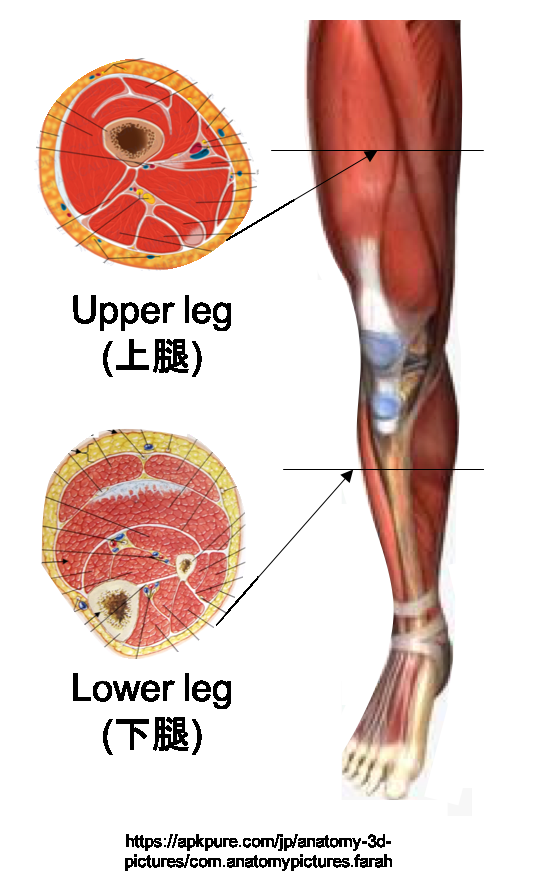
\includegraphics[width=50mm]{fig/kashisoshiki.pdf}
  \end{center}
  \caption{下肢組織の構造}
  \figlab{kashisoshiki}
\end{figure}
\section{シミュレーション}
\subsection{シミュレーション系の設定\label{simulationmodel}}
本研究は下肢組織を対象としているために\figref{daitai}, \figref{keikotsu},  \figref{hikotsu}に示すような3種のシミュレーション系を設定した. 計算領域は, 110mm$\times$110mmであり, グリッドサイズは0.21mm$\times$0.21mmである. また, 周波数は1.6MHz, 筋肉および皮下組織内の音速は1500m/s, 大腿骨, 脛骨および腓骨の音速は2700m/sとした(表\ref{simulation_settei}). 水中の音速は1500m/sであるが, まずはシミュレーションの条件を単純化するべく, 筋肉および皮下組織内の音速も1500m/sで近似している. そのため, 今回のシミュレーションでは水の中に骨のみがあるようなモデルでシミュレーションを行なった. \figref{daitai}, \figref{keikotsu},  \figref{hikotsu}を取り囲むように, 直径100mm, 圧電素子数1024のリング型アレイトランスデューサが設置されている. 
\begin{figure}[H]
 \begin{minipage}{0.325\hsize}
  \begin{center}
   \includegraphics[width=40mm]{fig/daitai.pdf}
  \end{center}
  \caption{大腿骨モデル}
   \figlab{daitai}
 \end{minipage}
 \begin{minipage}{0.325\hsize}
 \begin{center}
  \includegraphics[width=40mm]{fig/keikotsu.pdf}
 \end{center}
  \caption{脛骨モデル}
  \figlab{keikotsu}
 \end{minipage}
 \begin{minipage}{0.325\hsize}
 \begin{center}
  \includegraphics[width=40mm]{fig/hikotsu.pdf}
 \end{center}
  \caption{脛骨・腓骨モデル}
  \figlab{hikotsu}
 \end{minipage}
\end{figure}
\begin{table}[H]
\centering
\caption{シミュレーション系の設定}
\label{simulation_settei}
\begin{tabular}{|c|c|c|}
\hline
組織 & 直径[mm] & 計測周波数$f$[Hz]  \\ \hline
筋肉 & - &      1500 \\ \hline
皮下組織   & - &      1500\\ \hline
大腿骨  & 30 &     2700 \\ \hline
脛骨 & 30 &     2700 \\ \hline
腓骨  & 7 &     2700  \\ \hline
\end{tabular}
\end{table}
\subsection{k-Wave}
本研究では, 筋肉や腱を模した実験系から得たRF信号を処理することで,再構成画像を得るが, 同時に画像再構成の解像度の向上を目指す. そこで, まずは超音波の伝播のシミュレーションを行う. シミュレーションで用いるソフトウェアはk-Waveで, MATLABのtoolboxである. k-Waveの基礎方程式は, %式の扱いをどうするか
%連続の式((\ref{eq.renzoku})式)および波動方程式((\ref{eq.hadou})式)である. 
\begin{equation}
\label{eq.renzoku}
\\\ \frac{\partial \textbf{u}}{\partial t} = - \frac{1}{\rho_0} \nabla p
\end{equation}
\begin{equation}
\label{eq.renzoku}
\\\ \frac{\partial \rho}{\partial t} = - \rho_0 \nabla p ・ \textbf{u}
\end{equation}\begin{equation}
\label{eq.renzoku}
\\\ p = c^2 \rho
\end{equation}
計算手法は擬似スペクトル法である. 以下で擬似スペクトル法について詳しく説明する. 
\subsection{k-space 擬似スペクトル法}
擬似スペクトル法は, 波動方程式の解の1種である. 1次元の波動方程式を用いて, 擬似スペクトル法について説明する. 波動方程式を, (\ref{eq.risan})式を用いて離散化する. 
\begin{equation}
\label{eq.risan}
\\\ \frac{{p_j} ^{n+1} - 2{p_j}^n + {p_j}^{n-1}} {\Delta t^2}= {c_0}^2 \frac{{p_{j+1}} ^n - 2{p_{j-1}}^n + p^n} {\Delta t^2}
\end{equation}
jは空間方向, nは時間方向のインデックスである. 安定条件は(\ref{eq.antei})式に示す.
\begin{equation}
\label{eq.antei}
\\\ \frac{c_0 \Delta t}{\Delta x} \leqq 1
\end{equation}
また, 打ち切り誤差の補正を(\ref{eq.uchikiri})式で行う. ただし, $c_0$は音速, $k$は波数である.
\begin{equation}
\label{eq.uchikiri}
\\\ c(k) = \dfrac{sinc \left(\dfrac{k \Delta x}{2} \right)}{sinc \left(\dfrac{c_0 k \Delta t}{2} \right)} c_0
\end{equation}
擬似スペクトル法は, 空間の離散化による誤差の低減のためにフーリエ変換を用いる. フーリエ変換では, 微分値の制度が差分法より優れており, グリッド数はより少なく済む. \cite{hayashisan[36]}, \cite{hayashisan[37]}. k-space擬似スペクトル法では, 時間方向の離散化による誤差の低減の補正項は(\ref{eq.kspacehosei})式で表せる.
\begin{equation}
\label{eq.kspacehosei}
\\\ \kappa = sinc \left(\dfrac{c_0 k \Delta t}{2} \right)
\end{equation}
(\ref{eq.kspacehosei})式を用いて, (\ref{eq.risan})式および(\ref{eq.antei})式はそれぞれ, (\ref{eq.gijirisan})式, (\ref{eq.gijiuchikiri})式に書き直せる. 
\begin{equation}
\label{eq.gijirisan}
\\\ \frac{{p_j} ^{n+1} - 2{p_j}^n + {p_j}^{n-1}} {\Delta t^2}= {c_0}(k)^2 \mathcal{F}^{-1}\{ {-\kappa}^2 {k_x}^2  \mathcal{F}(p^n)\} 
\end{equation}
\begin{equation}
\label{eq.gijiuchikiri}
\\\ c_0(k) = \frac{1}{sinc \left(\dfrac{c_0 k \Delta t}{2} \right)} c_0
\end{equation}
これにより, タイムステップは大きく向上した.
\subsubsection{完全整合層}
k-space擬似スペクトル法では, 計算領域を周期的なものと仮定している. そのため, 領域から出た出て行く波が反対側から入射するような現象が起こる. 完全整合層は, そのような問題を解決する吸収境界条件のことである\cite{hayashisan[38]}, \cite{hayashisan[39]}. 
\subsubsection{スタッガードグリッド}
スタッガードグリッドとは, 変数ごとの定義点を1/2グリッドずつずらす手法である. スタッガードグリッドを用いることで, k-space 擬似スペクトル法での正確性や安定性が向上する\cite{hayashisan[42]}. \figref{stagado}に, スタッガードグリッドの概念図を示す. ただし, ($x, z$) における音圧$p$から算出される粒子速度$u_x$, $u_y$はそれぞれ ($x+\Delta x /2, z$),  ($x, z + \Delta z /2$)の粒子速度として割り当てる. したがって, 音圧$p$の変化に伴い隣接する粒子速度は直接影響を受ける. 
\begin{figure}[h]
  \begin{center}
    \includegraphics[width=65mm]{fig/stagado.pdf}
  \end{center}
  \caption{スタッガードグリッドの概念図}
  \figlab{stagado}
\end{figure}
\subsection{下肢組織に対する超音波伝播シミュレーション}
下肢組織を模したモデルに対して超音波伝播シミュレーションを行った. 送信素子は16素子, 受信素子は1024素子である. 超音波の周波数は1.6MHz, アレイ半径は50mmである. \figref{zantei}は, 第\ref{simulationmodel}項で示した3つのモデルのうち, 大腿骨モデルのシミュレーションにおいて超音波が伝播して行く様子を示したものである. 
\begin{figure}[H]
 \begin{minipage}{0.5\hsize}
  \begin{center}
   \includegraphics[width=40mm]{fig/daitai.pdf}
  \end{center}
%  \caption{大腿骨モデル}
   \figlab{daitai}
 \end{minipage}
 \begin{minipage}{0.5\hsize}
 \begin{center}
  \includegraphics[width=40mm]{fig/keikotsu.pdf}
 \end{center}
%  \caption{脛骨モデル}
  \figlab{keikotsu}
 \end{minipage}
 \end{figure}
 \begin{figure}[H]
 \begin{minipage}{0.5\hsize}
  \begin{center}
   \includegraphics[width=40mm]{fig/daitai.pdf}
  \end{center}
%  \caption{大腿骨モデル}
   \figlab{daitai}
 \end{minipage}
 \begin{minipage}{0.5\hsize}
 \begin{center}
  \includegraphics[width=40mm]{fig/keikotsu.pdf}
 \end{center}
%  \caption{脛骨モデル}
  \figlab{keikotsu}
 \end{minipage}
 \end{figure}
\begin{figure}[h]
  \begin{center}
    \includegraphics[width=110mm]{fig/zantei.pdf}
  \end{center}
  \caption{超音波伝播シミュレーション}
  \figlab{zantei}
\end{figure}
\subsection{画像再構成のアルゴリズム}
超音波シミレーションで得た, エコーデータから再構成画像を生成するアルゴリズムについて詳しく説明する\cite{cure1}. \figref{echodata1soshi}は, エコーデータの一例である. 横軸は受信素子を表し, 縦軸は到達時間を表している. 到達時間$\tau$は(\ref{eq.toutatsu})式で算出される. ただし. $l_T$は送信素子と散乱体との距離, $l_R$は受信素子と散乱体との距離である. 
\begin{equation}
\label{eq.toutatsu}
\\\ \tau = \dfrac{l_T + l_R}{v}
\end{equation}
送信素子から送波された超音波が散乱体によって反射され受信素子に届くまでの距離の総和を音速で割ることで到達時間が求められる. 
 \begin{figure}[H]
  \begin{center}
    \includegraphics[width=80mm]{fig/echodata1soshi.pdf}
  \end{center}
  \caption{エコーデータ}
  \figlab{echodata1soshi}
\end{figure}
\figref{echodata1soshi}で示したように, 到達時間は受信素子番号の関数として表現でき, 関数の曲線上のエコーデータの信号値を足し合わせると, その総和が仮定した散乱体の位置における反射強度になる. したがって, 仮定した散乱体の位置と真の散乱体の位置が一致すると, 反射強度は最大になる. 
%透過波を除いた形になってしまうがそれはなぜなのかを書く
\subsection{16の送信素子に対する輝度値マッピングと合成}
本研究でのシミュレーションでは, 送信素子は16素子になっているが, それぞれにおいて再構成画像を作成し, 輝度値をマッピングすることができる. 16素子それぞれに対する再構成画像をさらに重ね合わせて1枚の画像を作り出すことで, 散乱体の信号をより強調する画像ができる. 送信素子の数が増加するほどより正確な散乱体のマッピングができるが, 計算コストも増加する. そのため本研究では16素子から1枚の再構成画像を作成した. \figref{daitai16}\verb|〜|\figref{hikotsu16}は, 各送信素子に対して得た再構成画像と, それらを重ね合わせた再構成画像を第\ref{simulationmodel}項で述べた3種のシミュレーションモデルに対して作成したものである. シミュレーションモデルに対して, 概ね一致した場所に散乱体のマッピングができていることがわかるが, その正確性については後述する. 
\begin{figure}[H]
  \begin{center}
    \includegraphics[width=90mm]{fig/daitai16.pdf}
  \end{center}
  \caption{大腿骨モデルに対する再構成画像}
  \figlab{daitai16}
\end{figure}
\begin{figure}[H]
  \begin{center}
    \includegraphics[width=90mm]{fig/keikotsu16.pdf}
  \end{center}
  \caption{脛骨モデルに対する再構成画像}
  \figlab{keikotsu16}
\end{figure}
\begin{figure}[H]
  \begin{center}
    \includegraphics[width=90mm]{fig/hikotsu16.pdf}
  \end{center}
  \caption{脛骨・腓骨モデルに対する再構成画像}
  \figlab{hikotsu16}
\end{figure}
\subsection{再構成画像の解析}
シミュレーションで得られた再構成画像の散乱体の位置と, 真の散乱体の位置との差異を解析, 検討する. 
\subsection{再構成画像の解像度の向上と統計的処理}
k-Waveシミュレーションにおいて再構成画像にアーチファクトが生じる原因としては, 以下の2つが考えられる. 
\begin{enumerate}
\item 散乱体が離散的ではなく, 連続的に処理される. 
\item 多重反射が起こる.  
\end{enumerate}
本研究では, 多重反射に着目して再構成画像の解像度の向上を目指す. 本研究でのシミュレーションモデルでは, 水の中に大腿骨, 脛骨, 腓骨などの骨がある系になっている. そのため, 各送信条件においての受信素子の信号値にもばらつきが出る. 脛骨・腓骨モデルについて\figref{hikotsusaikousei}で示すように, 再構成画像から3点をランダムに選び, 各送信条件に対する信号値のデータのばらつきを考察した.
\begin{figure}[H]
  \begin{center}
    \includegraphics[width=140mm]{fig/hikotsusaikousei.pdf}
  \end{center}
  \caption{脛骨・腓骨モデルに対する再構成画像}
  \figlab{hikotsusaikousei}
\end{figure}
\figref{kaiseki3data}は, 前述した3点について16の送信素子に対する反射強度の正規分布である. \figref{kaiseki3data}で示されるように, 散乱体がない座標[112, 211]では正規分布が細長く分布しているが, 座標[256, 182]あるいは座標[362, 131]では散乱体がない場所に比べて正規分布の裾野が広くなっている. これは, 散乱体がある場合には各送信素子に対する信号値が様々な値をとるからである. 例えば, 散乱体から近い場所に送信素子がある場合と, 遠い場所に送信素子がある場合には各受信素子が受け取る信号値の値が異なる. 一方, 散乱体がない場所には送信素子の場所に関わらず, 信号値のばらつきが小さくなる. 
 %反射強度の単位をしっかりかく
\begin{figure}[H]
  \begin{center}
    \includegraphics[width=90mm]{fig/kaiseki3data.pdf}
  \end{center}
  \caption{脛骨・腓骨モデルに対する再構成画像}
  \figlab{kaiseki3data}
\end{figure}
%アーチファクトの説明がいるかな
したがって, 以下では再構成画像上のランダムな点の各送信素子に対する, データのばらつきを正規分布で整理することによって, 散乱体の有無を判断する手法を考案する. 本研究で行なった手法は, 再構成画像における散乱体の有無に対してある標準偏差の閾値を決め, その閾値を超える座標には散乱体があると判断する. また, 標準偏差の値が閾値を超えない場合は, 散乱体が無いと判断し, 信号値の値を0に変更する. 閾値の設定方法は, \\
\ \ \ \figref{gassanhikaku}は, 再構成画像の信号値に統計的処理を行い, 散乱体のマッピングの画像を再構成し直したものである. 左が統計的処理を加える前で, 右が統計的処理を加えた後の再構成画像である. 上段から大腿骨モデル, 脛骨モデル, 脛骨・腓骨モデルの比較である. 
%正規分布のばらつきについての指標の検討方法を考える. 
\begin{figure}[H]
  \begin{center}
    \includegraphics[width=140mm]{fig/gassanhikaku.pdf}
  \end{center}
  \caption{統計的処理による再構成画像との比較}
  \figlab{gassanhikaku}
\end{figure}
%デシベル表記してることも示す必要がある. 
%脛骨・腓骨モデル以外が閾値が標準偏差0.2になっている可能性がある. 
両者の反射強度の比較, 改善度を定量的に示す. 
\ \ \ また, 大腿骨モデルおよび脛骨モデルに関しては, 元の再構成画像に比べ輪郭がよりはっきりとプロットされている. 一方, 脛骨・腓骨モデルに関しては, 脛骨と腓骨の間の反射強度がシミュレーションモデル通り出ていないことがわかる. そのため, 反射強度が小さい部分に対して角度方向に反射強度をプロットしてマッピングの妥当性を図る. 